\documentclass{article}
\linespread{1.3}
\usepackage[margin=50pt]{geometry}
\usepackage{amsmath, amsthm, amssymb, amsthm, tikz, fancyhdr}
\pagestyle{fancy}
\renewcommand{\headrulewidth}{0pt}
\newcommand{\changefont}{\fontsize{15}{15}\selectfont}

\newcommand{\field}[1]{\mathbb{#1}}
\newcommand{\1}{\mathbf{1}}
\newcommand{\E}{\mathbb{E}} 
\renewcommand{\P}{\mathbb{P}}
\newcommand{\R}{\field{R}} % real domain
% \newcommand{\C}{\field{C}} % complex domain
\newcommand{\F}{\field{F}} % functional domain

\newcommand{\T}{^{\textrm T}} % transpose

\def\diag{\text{diag}}

%% operator in linear algebra, functional analysis
\newcommand{\inner}[2]{#1\cdot #2}
\newcommand{\norm}[1]{\left\|#1\right\|}
\newcommand{\twonorm}[1]{\|#1\|_2^2}
% operator in functios, maps such as M: domain1 --> domain 2
\newcommand{\Map}[1]{\mathcal{#1}}
\renewcommand{\theenumi}{\alph{enumi}} 

\newcommand{\Perp}{\perp \! \! \! \perp}

\newcommand\independent{\protect\mathpalette{\protect\independenT}{\perp}}
\def\independenT#1#2{\mathrel{\rlap{$#1#2$}\mkern2mu{#1#2}}}
\newcommand{\vct}[1]{\boldsymbol{#1}} % vector
\newcommand{\mat}[1]{\boldsymbol{#1}} % matrix
\newcommand{\cst}[1]{\mathsf{#1}} % constant
\newcommand{\ProbOpr}[1]{\mathbb{#1}}
\newcommand{\points}[1]{\small\textcolor{magenta}{\emph{[#1 points]}} \normalsize}
\date{{}}

\fancypagestyle{firstpageheader}
{
  \fancyhead[R]{\changefont Michael Huang \\ CSE 446 \\ Homework 2}
}

\begin{document}

\thispagestyle{firstpageheader}

\section*{Collaborators}
{\Large 
Jimmy Guo, Neil Kagalwala, Andrew Wang
}

\section*{A.0}
{\Large 

\subsection*{a.}

If we removed this feature that had large positive weight and refit the model, then the new model wil not necessarily have strictly higher error than before. It could have the same or even better prediction in a case such as if there is another better predictive feature that would increase in weight once we remove the feature with a large positive weight.

\subsection*{b.}

% An L1 norm penalty is more likely to result in sparsity in the weight vector since it will linearly decrease towards 0 with each step, which means that it will actually reach 0, which is not the case with the quadratic steps towards 0. L1 is therefore more likely to zero out coefficients.
The L1 optimum is more shaped like a diamond with points on the axes rather than the L2 optimum's smooth circle shape. The circle shape will only ever intersect with the isocountours of the LS objective only when its minimum point is exactly on the axis, while the pointy diamond shape are much more likely to intersect with the isocontours, at points other than when the minimum point is on the axis.

\subsection*{c.}

% One possible upside is that it is that features will tend to be zeroed out less often, which maintains these features' input in the model. \\ 
% One possible downside is that weights will tend to be larger for features that are less relevant, since we don't get as large gradients and changes when we perform regularization, especially when we near zero.
One possible upside is that it is that features will tend to be zeroed out more often, encouraging sparsity in our model that will make it easier to work with. \\ 
One possible downside is with fewer nonzero weights, the model might not be as accurate since it will be simpler with less relevant parameters.

\subsection*{d.}

True. If the step-size for gradient descent is too large, then it may diverge. This is because with a step size that is too large, then the values may overshoot and oscillate around an optimal point rather than generally converge upon it, as it normally would.

\subsection*{e.}

% Stochastic gradient descent iteratively chooses random samples from training data to update parameters. By randomly approximating the distribution dataset around the chosen random sample, we can effectively guess the gradients and update the weights based on the attributes of the distribution each time rather than having to run through all the data.
Stochastic gradient descent works since the gradient calculated from SGD is an unbiased estimator for the gradient from GD, which means that over time, the SGD will also converge towards the minimum.

\subsection*{f.}

An advantage of SGD over GD since you don't need to run through all samples in a set of training data, and save compute time overall. \\ 
A disadvantange of SGD relative to GD might be that the optimal point might not be found as quickly as with GD, and therefore require more iterations to get to the same minimum.

}

\section*{A.1}
{\Large

\subsection*{a.}

We aim to prove that $f(x) = \left( \sum_{i=1}^n |x_i| \right)$ is a norm. \\ \\
$(i)$ We start with showing non-negativity. \\
We first take the absolute value for each $x_i$ contained within $x$, and we know that \\
$|x_i| \geq 0$ $|_{i = 1, \dots, n}$ \\
We also know that the sum of non-negative elements will also be non-negative, which in turn tells us that \\ 
$\sum_{i=1}^{n} |x_i| \geq 0$ \\
We also need to show that if and only if $x = 0$, $\|x = 0\|$. \\
First, we know that if $x = 0$, then $|x| = 0$ as we know that since each $x_i = 0$,  \\
$|x_i| = |0| = 0$ $|_{i = 1, \dots, n}$ \\
which in turn tells us that \\ 
$\sum_{i=1}^{n} |x_i| = \sum_{i=1}^{n} |0| = 0$ \\
Then, we need to show the other direction; that is, if and only if $\|x\| = 0$, $x = 0$. By the contrapositive, we can say that if $x \neq 0$, then $\|x\| \neq 0$. If $x \neq 0$, then we know that as we now know through absolute value, \\
$|x_i| > 0 |_{i = 1, \dots, n}$ \\
which in turn using addition tells us that  \\ 
$\sum_{i=1}^{n} |x_i| > 0 \neq 0$ \\
which is exactly what we sought to show. \\ \\
$(ii)$ We then look at absolute scalability. By definition, \\
$\|ax\| $ \\
$ = (\sum_{i=1}^{n} |ax_i|)$ \\
$ = (\sum_{i=1}^{n} |a| |x_i|)$ \\
$ = (|a| \sum_{i=1}^{n} |x_i|)$ \\
$ = |a| (\sum_{i=1}^{n} |x_i|)$ \\
$ = |a| \|x\|$ \\
which is exactly what we sought to show. \\ \\
$(iii)$ Finally, we look at the triangle inequality. We begin by showing that $|a + b| \leq |a| + |b|$ for all $a, b \in \R$: \\
$|a + b| \leq |a| + |b|$ \\
$(|a + b|)^2 \leq (|a| + |b|)^2$ \hfill Square both sides \\
$a^2 + b^2 + 2ab \leq a^2 + b^2 + 2|a||b|$ \\
$2ab \leq 2|ab|$ \\
$ab \leq |ab|$ \\ 
We can see that this statement is true since if $a$ and $b$ are both positive or both negative, then the two sides are equal. However, in the case that $a$ and $b$ are of opposite signs, then we can see that although the magnitudes of both sides will be equal, the left side will be negative, and the right side will be positive, which makes the left side less than the right side. \\
We can then go on to use this in proving the statement: \\
$\|x + y\| $ \\ 
$= (\sum_{i=1}^{n} |x_i + y_i|) $ \\
$\leq (\sum_{i=1}^{n} |x_i| + |y_i|) $ \hfill Using what we proved \\
$\leq (\sum_{i=1}^{n} |x_i| + \sum_{i=1}^{n} |y_i|) $ \\
$\leq (\sum_{i=1}^{n} |x_i|) + (\sum_{i=1}^{n} |y_i|) $ \\
$\leq \|x\| + \|y\|$ \\
which is exactly what we sought to show. \\ \\
Since we have proved that all 3 properties hold for $f(x)$, we can see that it is indeed a norm. 

\subsection*{b.}

We aim to show that $g(x) = \left(\sum_{i=1}^n |x_i|^{1/2}\right)^2$ is not a norm, which we can easily show using a counterexample. If we take two $n=2$ dimensional plants $x = (1, 9)$ and $y = (16, 0)$, we see that the triangle inequality does not hold: \\
$\| x \| = (|1^{1/2}| + |9^{1/2}|)^2 = (1 + 3)^2 = 4^2 = 16$ \\ 
$\| y \| = (|16^{1/2}| + |0^{1/2}|)^2 = (4 + 0)^2 = 16$ \\ \\
$\|x + y\| \leq \|x\| + \|y\|$ \\ 
$((1 + 9)^{1/2} + (16 + 0)^{1/2})^2 \leq 16 + 16$ \\ 
$(\sqrt{10} + 4)^2 \leq 32$ \\ 
$10 + 16 + 8\sqrt{10} \leq 32$ \\ 
$26 + 8\sqrt{10} \leq 32$ \\ 
$\sim 51.30 \leq 32$ \\ 
which is false and shows that the triangle inequality does not hold, which tells us that $g(x)$ is indeed not a norm.

\newpage

}

\section*{A.2}
{\Large 

\subsection*{I}
Not convex. We see that connecting point $b$ to $c$ results in a line outside of the grey shaded set.

\subsection*{II}
Convex. We see that any line that we draw between points stays within the shaded set.

\subsection*{III}
Not convex. We can see that connecting point $d$ to $a$ would result in a line outside of the grey shaded set.

\newpage

}

\section*{A.3}
{\Large 

\subsection*{a.}

The function is convex, as we see that any connections between points are contained above the function.

\subsection*{b.}

The function is not convex. It is possible to connect lines between points that are below the function, such as from point $a$ to $b$ or from point $b$ to $c$.

\subsection*{c.}

The function is not convex. It is possible to connect lines between points that will have sections below the function, such as from point $a$ to any other point on the interval.

\subsection*{d.}

The function is convex, since any connections between points would be constructed above the function.

\newpage

}

\section*{A.4}
{\Large 

\begin{verbatim}
# lasso.py
# A4: Lasso implementation

import matplotlib.pyplot as plt
import numpy as np

import constants as c
import helpers as h

def main():
  print("binary logistic regression")

  lamb_data = []
  nonzero_data = []

  fdr_data = []
  tpr_data = []

  lasso = Lasso()

  lasso.generate_synthetic_data()
  lamb = h.min_lamb(lasso.X, lasso.Y)

  n, d = lasso.X.shape
  k = 100

  w = np.zeros((d, 1))

  # abritrarily stop when we hit 995/1000
  while np.count_nonzero(w) < d - 5:
    # print("lasso lambda value: " + str(lamb))

    # perform coordinate descent 
    w, _ = lasso.coord_desc(lamb)

    # append lambda/nonzero data
    lamb_data.append(lamb)
    nz_count = np.count_nonzero(w)
    nonzero_data.append(nz_count)

    # update lambda
    lamb = lamb / 2

    # append fdr/tpr data
    if k == 0 or nz_count == 0:
      continue

    fdr_data.append(np.count_nonzero(w[k:]) / nz_count)
    tpr_data.append(np.count_nonzero(w[:k]) / k)

  h.plot_single("Nonzero Coefficients over Lambda", "a4_a",
                "Lambda", "Nonzero Coefficients", lamb_data, nonzero_data, True)

  h.plot_single("TPR over FDR", "a4_b",
                "FDR", "TPR", fdr_data, tpr_data)

class Lasso:
  def __init__(self, X=None, Y=None):
    self.X = X
    self.Y = np.squeeze(Y)

  def coord_desc(self, lamb, cutoff=c.cutoff, w=None):
    assert (self.X is not None), "We need to have some X or else our dimensions fail"

    n, d = self.X.shape

    b = 0
    a = 2 * np.sum(np.square(self.X), axis=0)
    c = np.zeros((d, 1))

    if w is None:
      w = np.zeros((d, 1))

    while True:
      w_diff = 0

      w = np.squeeze(w)
      wx_sum = (w.T).dot(self.X.T)
      b = (1 / n) * np.sum(self.Y - wx_sum)
      
      for k in range(d):
        old_w = w[k]

        # only include where j =/= k, so subtract that
        wx_neqk_sum = (w.T).dot(self.X.T) - np.multiply(w[k], self.X[:, k])

        c[k] = 2 * self.X[:, k].dot(self.Y - (b + wx_neqk_sum))

        if c[k] < -lamb:
          w[k] = (c[k] + lamb) / a[k]
        elif c[k] > lamb:
          w[k] = (c[k] - lamb) / a[k]
        else: 
          w[k] = 0

        if np.abs(w[k] - old_w) > w_diff:
          w_diff = np.abs(w[k] - old_w)

      if w_diff < cutoff:
        break
    
    return w, b

  def generate_synthetic_data(self, n=500, d=1000, k=100, sd=1):
    print("generating synthetic data")

    w = list(range(1, k + 1))
    w.extend(np.zeros(d - len(w)))
    w = np.expand_dims(w, axis=1)
    w = w / k
    
    X = np.random.normal(size=(n, d))
    offset = np.random.normal(scale=sd, size=(n, ))
    Y = (w.T).dot(X.T) + offset

    self.X = X
    self.Y = np.squeeze(Y)

  def get_sqerror(self, w, b):
    assert (self.X is not None), "We need to have some X or else our dimensions fail"

    n, d = self.X.shape

    # print(w.shape)
    # print(self.X.shape)

    # print(((w.T).dot(self.X.T)).shape)

    Y_pred = (w.T).dot(self.X.T) + np.expand_dims(b, axis = 1)
    
    # print(Y_pred.shape)
    # print((np.square(Y_pred - self.Y)).shape)

    return (1 / n) * np.sum(np.square(Y_pred - self.Y), axis = 1)

if __name__ == "__main__":
  main()

\end{verbatim}

\subsection*{c.}

In general, having larger $\lambda$ means that we will have more zero-value weights in $w$, which makes sense since Lasso tends to encourage sparsity. We also see that larger $\lambda$ leads to lower TPR since we have fewer non-zero coefficients to err on, and thus also have lower FDR.

\newpage

\subsection*{a.}

\begin{figure}[h]
  \centering
  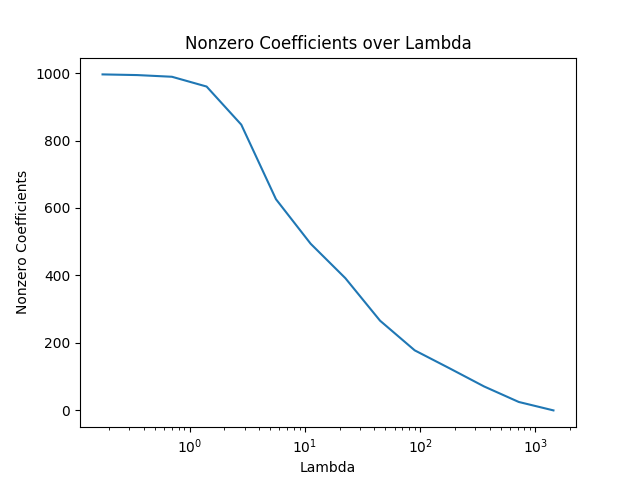
\includegraphics[width=120mm]{../hw2-code/results/a4_a.png}
\end{figure}

\subsection*{b.}

\begin{figure}[h]
  \centering
  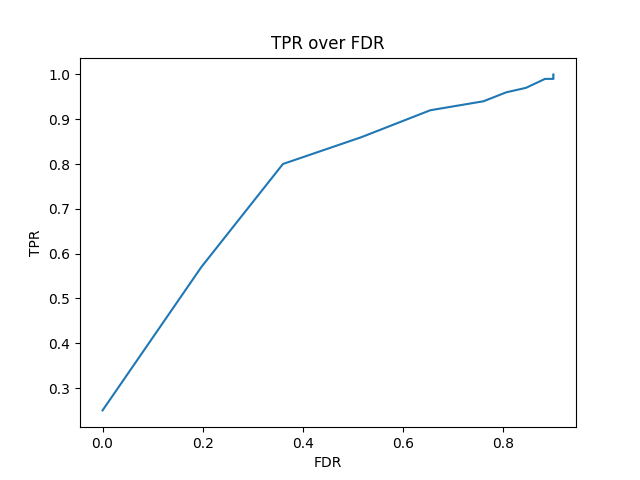
\includegraphics[width=120mm]{../hw2-code/results/a4_b.png}
\end{figure}

\newpage

}

\section*{A.5}
{\Large 

\begin{verbatim}
# crime-lasso.py
# A5: Application of Lasso to crime data

import matplotlib.pyplot as plt
import numpy as np
import pandas as pd

from tabulate import tabulate

import constants as c
import helpers as h
import lasso

def main():
  print("binary logistic regression")

  df_train, df_test = h.load_crime()

  X_train = df_train.iloc[:, 1:].values
  Y_train = df_train.iloc[:, :1].values

  X_test = df_test.iloc[:, 1:].values
  Y_test = df_test.iloc[:, :1].values

  input_indices = [df_train.columns.get_loc(col_name) for col_name in c.input_variables]

  lamb_data = []
  nonzero_data = []

  w_list = []
  b_list = []

  lamb = h.min_lamb(X_train, Y_train)

  crime_train_lasso = lasso.Lasso(X_train, Y_train)
  crime_test_lasso = lasso.Lasso(X_test, Y_test)

  w_zero = None

  while True:
    print("crime lasso lambda value: " + str(lamb))

    if w_zero is None:
      w_zero, b = crime_train_lasso.coord_desc(lamb)
      w = w_zero
    else:
      w, b = crime_train_lasso.coord_desc(lamb, w=w_zero)

    w_list.append(np.copy(w))
    b_list.append(b)

    lamb_data.append(lamb)
    nz_count = np.count_nonzero(w)
    nonzero_data.append(nz_count)

    if lamb < c.cutoff:
      break

    lamb = lamb / 2

  data_list = []
  for index in input_indices:
    data_list.append([w_list[i][index - 1] for i in range(len(w_list))])

  h.plot_single("Nonzero Coefficients over Lambda", "a5_c",
                "Lambda", "Nonzero Coefficients", lamb_data, nonzero_data, True)
  
  h.plot_multiple("Nonzero Coefficients over Lambda", "a5_d", "Lambda", "Weights", lamb_data, data_list, c.input_variables, True)

  train_sqerror_list = []
  test_sqerror_list = []

  w_list = np.array(w_list).T
  b_list = np.array(b_list)

  train_sqerror_list = crime_train_lasso.get_sqerror(w_list, b_list)
  test_sqerror_list = crime_test_lasso.get_sqerror(w_list, b_list)

  h.plot_function("Squared Error over Lambda", "a5_e",
                  "Lambda", "Squared Error", train_sqerror_list, test_sqerror_list, x_data=lamb_data, log_scale=True)

  lamb = 30
  if lamb == 30:
    # print("crime lasso lambda value: " + str(lamb))

    w30_train, b30_train = crime_train_lasso.coord_desc(lamb)
    w30_test, b30_test = crime_test_lasso.coord_desc(lamb)

    all_variables = df_train.columns[1:]

    nz_train = {all_variables[i]: w30_train[i]
                for i in range(len(w30_train)) if w30_train[i] != 0}
    nz_test = {all_variables[i]: w30_test[i]
               for i in range(len(w30_test)) if w30_test[i] != 0}

    output = open(c.results_path + "a5e" + c.txt_exten, "w")

    output.write("nonzero training weights\n")
    output.write(str(tabulate(nz_train.items())))
    
    output.write("\n\nnonzero test weights\n")
    output.write(str(tabulate(nz_test.items())))

    # find the min/max entries
    output.write("\n\ntraining min/max\n")
    min_train = min(nz_train, key=nz_train.get)
    output.write(min_train + " : " + str(nz_train.get(min_train)) + "\n")
    max_train = max(nz_train, key=nz_train.get)
    output.write(max_train + " : " + str(nz_train.get(max_train)) + "\n")

    output.write("\ntest min/max\n")
    min_test = min(nz_test, key=nz_test.get)
    output.write(min_test + " : " + str(nz_test.get(min_test)) + "\n")
    max_test = max(nz_test, key=nz_test.get)
    output.write(max_test + " : " + str(nz_test.get(max_test)) + "\n")

    output.close()


if __name__ == "__main__":
  main()

\end{verbatim}

\subsection*{a.}

\textbf{Number of homeless people counted in the street (NumStreet):} Homeless policies and laws affecting how homeless people are treated (e.g. a notable policy where homeless people in Eastside cities like Bellevue were forcibly transported to Seattle) can affect this number. \\
\textbf{Number of people under the poverty level (NumUnderPov):} There are a lot of different factors in policy that can affect poverty statistics: varied definitions of poverty as set by institutions, whether or how benefits are provided to the impoverished, cost of living standards and how that affects wages -- the list goes on and on. \\
\textbf{Mean people per household (householdsize):} The number of people per household can vary depending on the incentives that a family might receieve within their area for having children, as well as considering other factors that might affect their willingness to have children, such as employer policies in regards to maternity or paternity leave. \\

\subsection*{b.}

\textbf{Percentage of people 16 and over, in the labor force, and unemployed (PctUnemployed):} Unemployed people tend to be associated with crime, but one's able to become and stay employed might have been directly or indirectly affected by crime. \\
\textbf{Percentage of moms of kids 6 and under in labor force (PctWorkMomYoungKids):} Oftentimes, there is a bias against mothers who either are the breadwinners for the family or are not as present for the children leading to a tendency for their children to commit crime, however, this may not be true. \\
\textbf{Percent of people who do not speak English well (PctNotSpeakEnglWell):} People also associate immigrants or non-English speakers with crime, but this might not be accurate: these people are oftentimes those more targeted or  discriminated against when it comes to crime. \\

\subsection*{c.}

\begin{figure}[ht!]
  \centering
  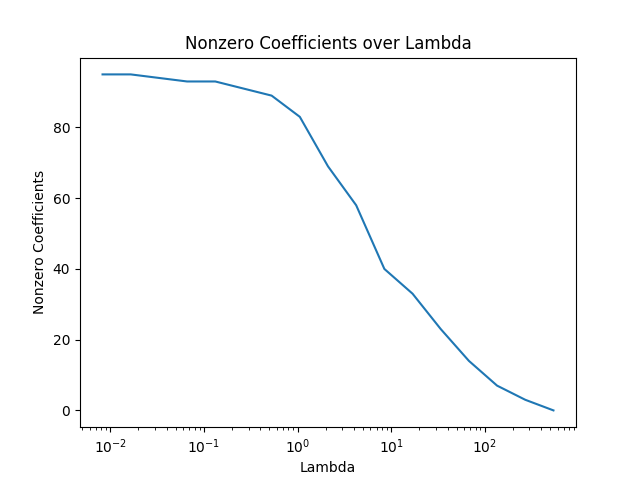
\includegraphics[width=180mm]{../hw2-code/results/a5_c.png}
\end{figure}

\newpage

\subsection*{d.}

\begin{figure}[ht!]
  \centering
  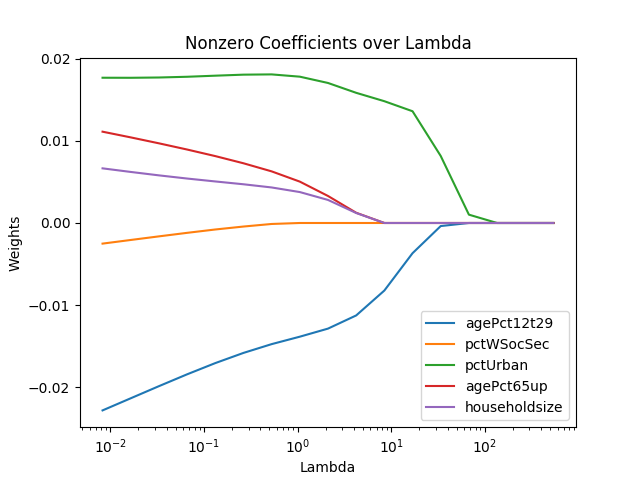
\includegraphics[width=120mm]{../hw2-code/results/a5_d.png}
\end{figure}

\subsection*{e.}

\begin{figure}[ht!]
  \centering
  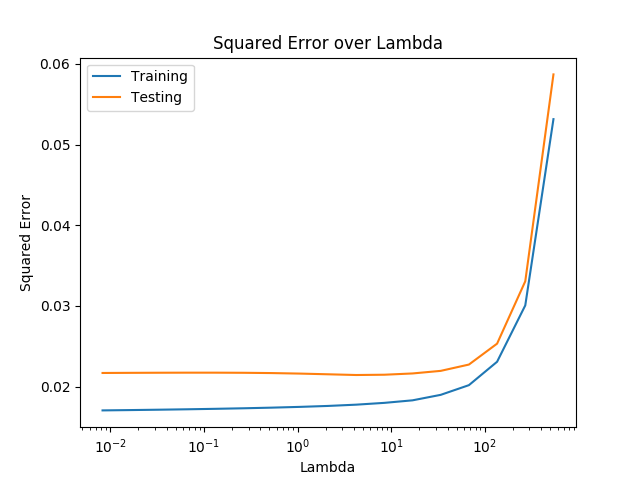
\includegraphics[width=120mm]{../hw2-code/results/a5_e.png}
\end{figure}

\newpage

\subsection*{f.}

\begin{verbatim}
nonzero training weights
---------------------  ------------
agePct12t29            -0.0063579
pctUrban                0.0125046
medIncome               0.000617753
pctWInvInc             -0.000866307
PctNotHSGrad            0.00176447
MalePctDivorce          0.00949172
PersPerFam              0.00363268
PctFam2Par             -0.0479927
PctKids2Par            -0.0371028
PctWorkMom             -0.00749318
PctIlleg                0.0633892
PctRecImmig10           0.00188808
PctLargHouseFam         0.0059379
PersPerRentOccHous      0.00110354
PctPersDenseHous        0.0190076
HousVacant              0.0200307
PctHousOccup           -0.00757211
MedOwnCostPctIncNoMtg  -0.00138742
NumStreet               0.0146808
PctForeignBorn          0.000664376
PctBornSameState       -0.000780591
---------------------  ------------

nonzero test weights
----------------  -----------
FemalePctDiv       0.0116801
PctFam2Par        -0.0659422
PctKids2Par       -0.0228941
NumIlleg           0.00624469
PctIlleg           0.0550029
PctPersDenseHous   0.00526577
----------------  -----------

training min/max
PctFam2Par : -0.04799273597230106
PctIlleg : 0.06338915717551429

test min/max
PctFam2Par : -0.06594215294586658
PctIlleg : 0.05500293686818547

\end{verbatim}

The most positive coefficient was found with the feature PctIlleg, which represents the percentage of kids born to never married parents. This an interesting finding since there is the stereotype that single parents, usually being the sole breadwinner in their family, aren't as present around children and can lead to delinquency over time. However, this might not necessarily be true and there could be other factors with the parents themselves that create this kind of positive relationship with violent crime. \\
The most negative coefficient was found with the feature PctFam2Par, which represents the percentage of families with 2 parents. This tells us that there was a relatively strong negative link between more families with 2 parents and level of crime, which means that there was a tendency for areas with more 2-parent families to have less crime. I feel like this might be categorized as causation, but I think it could be in the opposite way; that is, 2-parent families might tend to live in areas with less crime rather than the presence of 2-parent families leading to less crime. 

\subsection*{g.}

The issue with this line of reasoning is that correlation implies causation, which is not necessarily true. The fact that having greater population over the age of 65 is linked to lower crime might be true, but one may not necessarily cause the other. 

\newpage

}

\section*{A.6}
{\Large 

\subsection*{a.}

$J(w,b) = \frac{1}{n} \sum_{i=1}^n \log( 1 + \exp(-y_i (b + x_i^T w))) + \lambda ||w||_2^2$ \\
$\nabla_w J(w,b) = \nabla_w [\frac{1}{n} \sum_{i=1}^n \log( 1 + \exp(-y_i (b + x_i^T w))) + \lambda ||w||_2^2]$ \\ 
$ = \nabla_w \frac{1}{n} \sum_{i=1}^n \log( 1 + \exp(-y_i (b + x_i^T w))) + \nabla_w \lambda ||w||_2^2$ \\ 
$ = \frac{1}{n} \sum_{i=1}^n \nabla_w \log( 1 + \exp(-y_i (b + x_i^T w))) + 2 \lambda w$ \\ 
$ = \frac{1}{n} \sum_{i=1}^n \frac{1}{1 + \exp(-y_i (b + x_i^T w))} \cdot \exp(-y_i (b + x_i^T w)) \cdot -y_i (x_i^T) + 2 \lambda w$ \\ 
$ = \frac{1}{n} \sum_{i=1}^n \frac{-y_i x_i^T \exp(-y_i (b + x_i^T w))}{1 + \exp(-y_i (b + x_i^T w))} + 2 \lambda w$ \\ 
$ = \frac{1}{n} \sum_{i=1}^n -y_i x_i^T \mu_i(w, b) \exp(-y_i (b + x_i^T w)) + 2 \lambda w$ \\ 
$ = \frac{1}{n} \sum_{i=1}^n -y_i x_i^T \mu_i(w, b) (\frac{1}{\mu_i(w, b)} - 1) + 2 \lambda w$ \\ 
$ = \frac{1}{n} \sum_{i=1}^n -y_i x_i^T \mu_i(w, b) (\frac{1}{\mu_i(w, b)} - \frac{\mu_i(w, b)}{\mu_i(w, b)}) + 2 \lambda w$ \\ 
$ = \frac{1}{n} \sum_{i=1}^n -y_i x_i^T \mu_i(w, b) \frac{1 - \mu_i(w, b)}{\mu_i(w, b)} + 2 \lambda w$ \\ 
\framebox[1.1\width]{\textbf{$\nabla_w J(w,b) = \frac{1}{n} \sum_{i=1}^n -y_i x_i^T (1 - \mu_i(w, b)) + 2 \lambda w$}} \\ \\
$J(w,b) = \frac{1}{n} \sum_{i=1}^n \log( 1 + \exp(-y_i (b + x_i^T w))) + \lambda ||w||_2^2$ \\
$\nabla_{b} J(w,b) = \nabla_{b} [\frac{1}{n} \sum_{i=1}^n \log( 1 + \exp(-y_i (b + x_i^T w))) + \lambda ||w||_2^2]$ \\
$ = \nabla_{b} \frac{1}{n} \sum_{i=1}^n \log( 1 + \exp(-y_i (b + x_i^T w))) + \nabla_{b} \lambda ||w||_2^2$ \\ 
$ = \frac{1}{n} \sum_{i=1}^n \nabla_{b} \log( 1 + \exp(-y_i (b + x_i^T w))) + 0$ \\ 
$ = \frac{1}{n} \sum_{i=1}^n \frac{1}{\log( 1 + \exp(-y_i (b + x_i^T w)))} \cdot \exp(-y_i (b + x_i^T w)) \cdot -y_i(1)$ \\ 
$ = \frac{1}{n} \sum_{i=1}^n -y_i \mu_i(w, b) \cdot \exp(-y_i (b + x_i^T w))$ \\ 
$ = \frac{1}{n} \sum_{i=1}^n -y_i \mu_i(w, b) \frac{1 - \mu_i(w, b)}{\mu_i(w, b)}$ \\ 
\framebox[1.1\width]{\textbf{$\nabla_{b} J(w,b) = \frac{1}{n} \sum_{i=1}^n -y_i (1 - \mu_i(w, b))$}}

\newpage

\subsection*{b.}

\begin{figure}[hb]
  \centering
  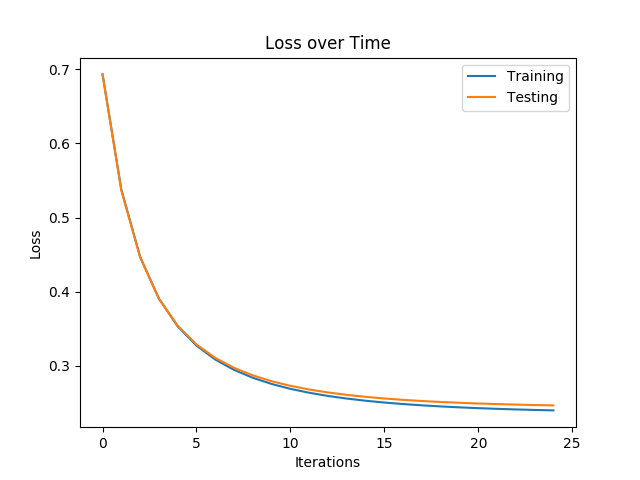
\includegraphics[width=120mm]{../hw2-code/results/a6_bi.png}
\end{figure}

\begin{figure}[h]
  \centering
  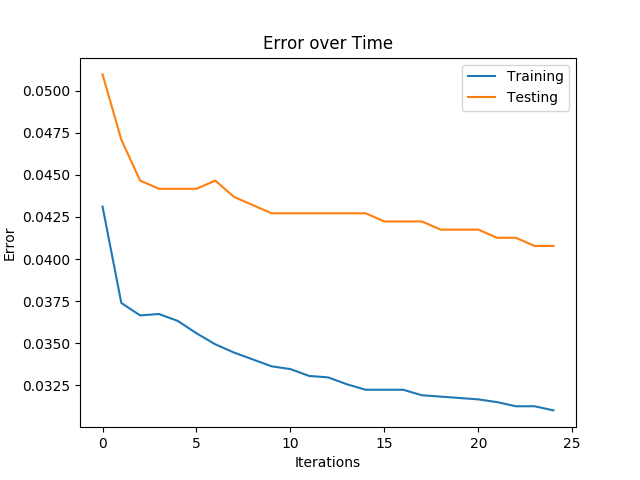
\includegraphics[width=120mm]{../hw2-code/results/a6_bii.png}
\end{figure}

\newpage

\subsection*{c.}

\begin{figure}[h]
  \centering
  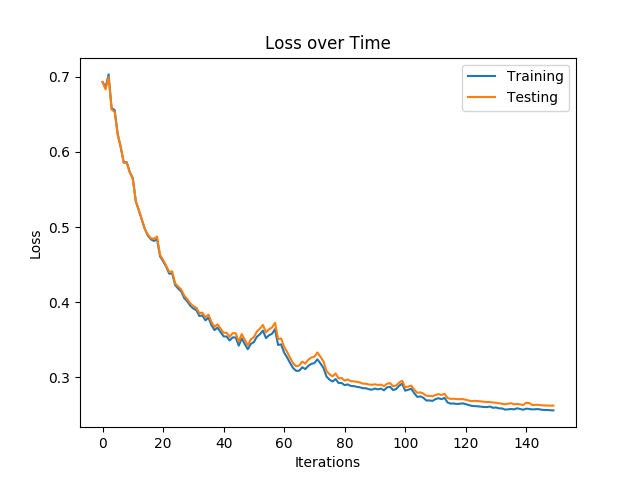
\includegraphics[width=120mm]{../hw2-code/results/a6_ci.png}
\end{figure}

\begin{figure}[h]
  \centering
  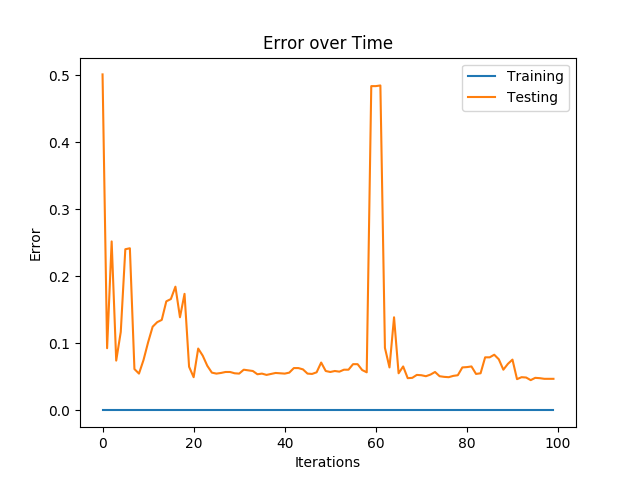
\includegraphics[width=120mm]{../hw2-code/results/a6_cii.png}
\end{figure}

\newpage

\subsection*{d.}

\begin{figure}[ht]
  \centering
  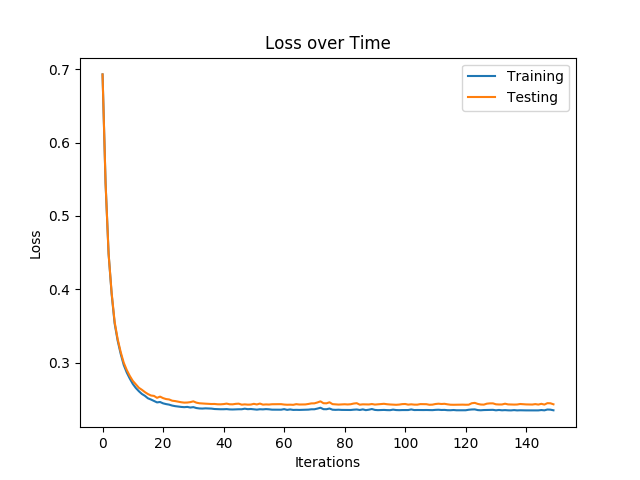
\includegraphics[width=120mm]{../hw2-code/results/a6_di.png}
\end{figure}

\begin{figure}[h]
  \centering
  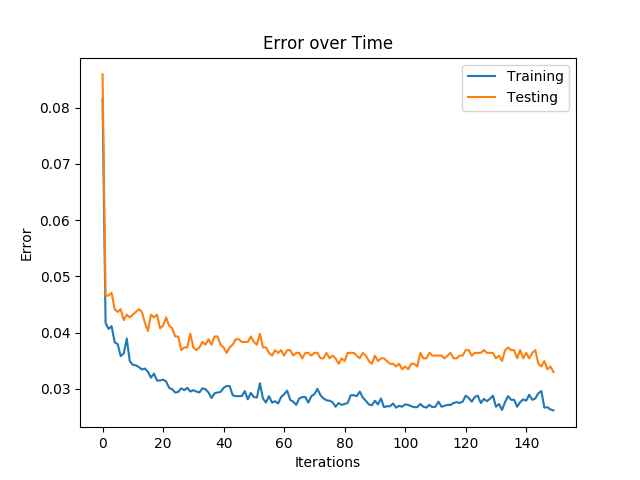
\includegraphics[width=120mm]{../hw2-code/results/a6_dii.png}
\end{figure}

\newpage

\begin{verbatim}
# binary-logistic.py
# A6: Binary logistic regression implementation

import matplotlib.pyplot as plt
import numpy as np
import random

import constants as c
import helpers as h

from scipy import linalg

# Run only what you need
run_b = True
run_c = True
run_d = True

def main():
  print("binary logistic regression")

  # Y-values are in [-1, +1] format
  X_train, labels_train, Y_train, X_test, labels_test, Y_test = h.load_mnist()

  assert (len(X_train) > 0 and len(X_test) > 0)
  
  # Gradient Descent

  if run_b:
    gd = GradientDescent(c.reg_lambda, c.mnist_step_size)
    train_j, test_j, train_error, test_error = gd.grad_desc(X_train, Y_train, X_test, Y_test, c.cutoff)

    h.plot_function("Loss over Time", "a6_bi", "Iterations", "Loss", train_j, test_j)
    h.plot_function("Error over Time", "a6_bii", "Iterations", "Error", train_error, test_error)

  # Stochastic Gradient Descent
  
  if run_c:
    sgd1 = StochasticGradientDescent(c.reg_lambda, c.mnist_step_size, 1)
    single_train_j, single_test_j, single_train_error, single_test_error = sgd1.stoch_grad_desc(
        X_train, Y_train, X_test, Y_test, c.cutoff)

    h.plot_function("Loss over Time", "a6_ci", "Iterations",
                    "Loss", single_train_j, single_test_j)
    h.plot_function("Error over Time", "a6_cii", "Iterations",
                    "Error", single_train_error, single_test_error)
    

  if run_d:
    sgd100 = StochasticGradientDescent(c.reg_lambda, c.mnist_step_size, 100)
    batch_train_j, batch_test_j, batch_train_error, batch_test_error = sgd100.stoch_grad_desc(
        X_train, Y_train, X_test, Y_test, c.cutoff)

    h.plot_function("Loss over Time", "a6_di",
                    "Iterations", "Loss", batch_train_j, batch_test_j)
    h.plot_function("Error over Time", "a6_dii", "Iterations",
                    "Error", batch_train_error, batch_test_error)

class GradientDescent:
  def __init__(self, reg_lambda, step_size):
    self.lamb = reg_lambda
    self.step = step_size
    self.w = None
    self.b = 0
    self.d = 0

  def grad_desc(self, X_train, Y_train, X_test, Y_test, cutoff=c.cutoff):
    print("gradient descent")
    
    # 12223, 784
    _, self.d = X_train.shape
    self.w = np.zeros((self.d, 1))

    train_j_data = []
    test_j_data = []
    train_class_data = []
    test_class_data = []

    # emulate do-while
    while True:

      train_j_func, grad_w, grad_b = self.get_j(X_train, Y_train)
      test_j_func, _, _ = self.get_j(X_test, Y_test)

      self.w = self.w - (self.step * grad_w)
      self.b = self.b - (self.step * grad_b)

      train_j_data.append(train_j_func[0][0])
      test_j_data.append(test_j_func[0][0])
      train_class_data.append(self.get_error(X_train, Y_train))
      test_class_data.append(self.get_error(X_test, Y_test))

      if max(np.max(np.abs(grad_w)), grad_b) < cutoff:
        break

    return train_j_data, test_j_data, train_class_data, test_class_data

  def get_j(self, X, Y):
    n, d = X.shape
    Y = np.expand_dims(Y, axis=1)

    offset = self.b + (self.w.T).dot(X.T)
    exponent = np.multiply(-Y, offset.T)
    mu = 1 / (1 + np.exp(exponent))

    reg = self.lamb * (self.w.T).dot(self.w)
    j_func = (1 / n) * np.sum(np.log(1 / mu)) + reg

    coef = np.multiply(X, -Y)
    grad_reg = 2 * self.lamb * self.w
    grad_w = (1 / n) * (coef.T).dot(1 - mu)
    grad_w = grad_w.sum(axis = 1)
    grad_w = np.expand_dims(grad_w, axis=1) + grad_reg

    grad_b = (1 / n) * (-Y.T).dot(1 - mu)

    return j_func, grad_w, grad_b[0][0]

  def get_error(self, X, Y):
    n, d = X.shape

    sign = np.sign(self.b + (self.w.T).dot(X.T))
    sign = sign[0]

    match_count = np.sum([sign[idx] == val for idx, val in enumerate(Y.T)])

    return 1 - (match_count / n)

class StochasticGradientDescent:
  def __init__(self, reg_lambda, step_size, batch_size):
    self.lamb = reg_lambda
    self.step = step_size
    self.batch = batch_size
    self.w = None
    self.b = 0
    self.d = 0

  # since it's random, maybe try capping an iter_count
  def stoch_grad_desc(self, X_train, Y_train, X_test, Y_test, cutoff=c.cutoff, iter_count=c.stoch_iter_count):
    print("stochastic gradient descent")

    n, self.d = X_train.shape
    self.w = np.zeros((self.d, 1))

    train_j_data = []
    test_j_data = []
    train_class_data = []
    test_class_data = []

    # emulate do-while
    for i in range(iter_count):
      indices = random.sample(range(n), self.batch)
      
      X_batch = X_train[indices]
      Y_batch = Y_train[indices]

      _, grad_w, grad_b = self.get_j(X_batch, Y_batch)
      train_j_func, _, _ = self.get_j(X_train, Y_train)
      test_j_func, _, _ = self.get_j(X_test, Y_test)

      self.w = self.w - (self.step * grad_w)
      self.b = self.b - (self.step * grad_b)

      train_j_data.append(train_j_func[0][0])
      test_j_data.append(test_j_func[0][0])
      train_class_data.append(self.get_error(X_train, Y_train))
      test_class_data.append(self.get_error(X_test, Y_test))

      if max(np.max(np.abs(grad_w)), grad_b) < cutoff:
        break

    return train_j_data, test_j_data, train_class_data, test_class_data

  def get_j(self, X, Y):
    n, d = X.shape
    Y = np.expand_dims(Y, axis=1)

    offset = self.b + (self.w.T).dot(X.T)
    exponent = np.multiply(-Y, offset.T)
    mu = 1 / (1 + np.exp(exponent))

    reg = self.lamb * (self.w.T).dot(self.w)
    j_func = (1 / n) * np.sum(np.log(1 / mu)) + reg

    coef = np.multiply(X, -Y)
    grad_reg = 2 * self.lamb * self.w
    grad_w = (1 / n) * (coef.T).dot(1 - mu)
    grad_w = grad_w.sum(axis = 1)
    grad_w = np.expand_dims(grad_w, axis=1) + grad_reg

    grad_b = (1 / n) * (-Y.T).dot(1 - mu)

    return j_func, grad_w, grad_b[0][0]

  def get_error(self, X, Y):
    n, d = X.shape

    sign = np.sign(self.b + (self.w.T).dot(X.T))
    sign = sign[0]

    match_count = np.sum([sign[idx] == val for idx, val in enumerate(Y.T)])

    return 1 - (match_count / n)

if __name__ == "__main__":
  main()

\end{verbatim}

\begin{verbatim}
# helpers.py
# Applicable helpers for HW2

import pandas as pd
import matplotlib.pyplot as plt
import numpy as np

import constants as c

from mnist import MNIST
from scipy import linalg

"""
Helper function for loading in MNIST data set
"""
def load_mnist():
  # load data
  mndata = MNIST(c.data_path)

  X_train, labels_train = map(np.array, mndata.load_training())
  X_test, labels_test = map(np.array, mndata.load_testing())
  X_train = X_train/255.0
  X_test = X_test/255.0

  # count number of 2s and 7s
  train_mask = np.logical_or(labels_train == 2, labels_train == 7)
  test_mask = np.logical_or(labels_test == 2, labels_test == 7)

  X_train = X_train[train_mask]
  X_test = X_test[test_mask]

  labels_train = labels_train[train_mask]
  labels_test = labels_test[test_mask]

  train_count = sum(labels_train == 2) + sum(labels_train == 7)
  test_count = sum(labels_test == 2) + sum(labels_test == 7)

  # convert labels to +/- 1
  one_train = np.zeros(train_count)
  one_test = np.zeros(test_count)

  for idx, train_val in enumerate(labels_train):
    one_train[idx] = c.digit_to_one[train_val]

  for idx, test_val in enumerate(labels_test):
    one_test[idx] = c.digit_to_one[test_val]

  return X_train, labels_train, one_train, X_test, labels_test, one_test

"""
Helper function for plotting function with training/testing distinction
"""
def plot_function(plt_title, img_title, x_label, y_label, train_data, test_data, x_data=None, log_scale=False):
  print("plot " + plt_title)

  if x_data is None:
    plt.plot(train_data)
    plt.plot(test_data)
  else:
    plt.plot(x_data, train_data)
    plt.plot(x_data, test_data)

  if log_scale:
    plt.xscale('log')

  plt.title(plt_title)
  plt.xlabel(x_label)
  plt.ylabel(y_label)
  plt.legend(["Training", "Testing"])

  plt.savefig(c.results_path + img_title + c.png_exten)
  plt.close()

"""
Helper function for plotting single function
"""
def plot_single(plt_title, img_title, x_label, y_label, x_data, y_data, log_scale=False):
  print("plot " + plt_title)

  plt.plot(x_data, y_data)

  plt.title(plt_title)
  plt.xlabel(x_label)
  plt.ylabel(y_label)

  if log_scale:
    plt.xscale('log')

  plt.savefig(c.results_path + img_title + c.png_exten)
  plt.close()

"""
Helper function for plotting multiple functions
"""
def plot_multiple(plt_title, img_title, x_label, y_label, x_data, data_list, legend_list, log_scale=False):
  print("plot " + plt_title)

  for data in data_list:
    plt.plot(x_data, data)

  plt.title(plt_title)
  plt.xlabel(x_label)
  plt.ylabel(y_label)
  plt.legend(legend_list)

  if log_scale:
    plt.xscale('log')

  plt.savefig(c.results_path + img_title + c.png_exten)
  plt.close()

"""
Helper function for getting min lasso lambda where w is all zero
"""
def min_lamb(X, Y):
  y_diff = Y.T - np.mean(Y)
  return np.max(2 * np.abs(y_diff.dot(X)))

"""
Helper function for loading in crime dataset
"""
def load_crime():
  df_train = pd.read_csv(c.data_path + "crime-train.txt", sep="\t")
  df_test = pd.read_csv(c.data_path + "crime-test.txt", sep="\t")

  return df_train, df_test

\end{verbatim}

\newpage

\begin{verbatim}
# constants.py
# Applicable constants for HW2

import numpy as np
import os

home_dir_path = os.path.dirname(os.path.dirname(os.path.abspath(__file__)))

data_path = home_dir_path + '/data/'
results_path = home_dir_path + '/results/'

png_exten = '.png'
txt_exten = '.txt'

reg_lambda = 1E-1

input_variables = ["agePct12t29", "pctWSocSec",
                   "pctUrban", "agePct65up", "householdsize"]

one_to_digit = { -1 : 2, +1 : 7}
digit_to_one = { 2 : -1, 7 : +1}

mnist_step_size = 1E-2
cutoff = 1E-2

stoch_iter_count = 150

\end{verbatim}

}

\end{document}